\documentclass[10pt,hyperref={CJKbookmarks=true},xcolor=dvipsnames,aspectratio=169]{beamer}
\usetheme[navigation]{UMONS}
\usepackage[utf8]{inputenc}
\usepackage{verbatim}
\usepackage{ctex}

\title[国际经济学]{国际经济学}
\subtitle{开放条件下的国民收入核算与国际收支平衡表}
\author{鲁晓东}
\institute[]{%
	岭南学院\hspace{2em}中山大学
	\\[4ex]
	
\includegraphics[height=8ex]{fig/lingnanlogo}\hspace{2em}%
	
\includegraphics[height=8.5ex]{fig/sysu}
}
%------------section前展示一页----------
\AtBeginSection[] {     
	\begin{frame}        
	\tableofcontents[currentsection,hideallsubsections]    
\end{frame} 
}

%-------------subsection也展示一下----------
\AtBeginSubsection[]{

\frame<beamer>{ 
	
	\frametitle{Outline}   
	
	\tableofcontents[currentsection,currentsubsection] 
	
}

}
%---------------------------

%-----------一段一闪现-------
%\beamerdefaultoverlayspecification{<+->}
%这个功能基本不用

\begin{document}
\maketitle


\begin{frame}
\frametitle{提纲}
\tableofcontents
\end{frame}				%生成提纲页

%-----------正文开始----------------------

%\beamerdefaultoverlayspecification{<+->}
\section{Motivation}

\begin{frame}{Beyond Barter:Not Just Trade in Commodities}
\centering
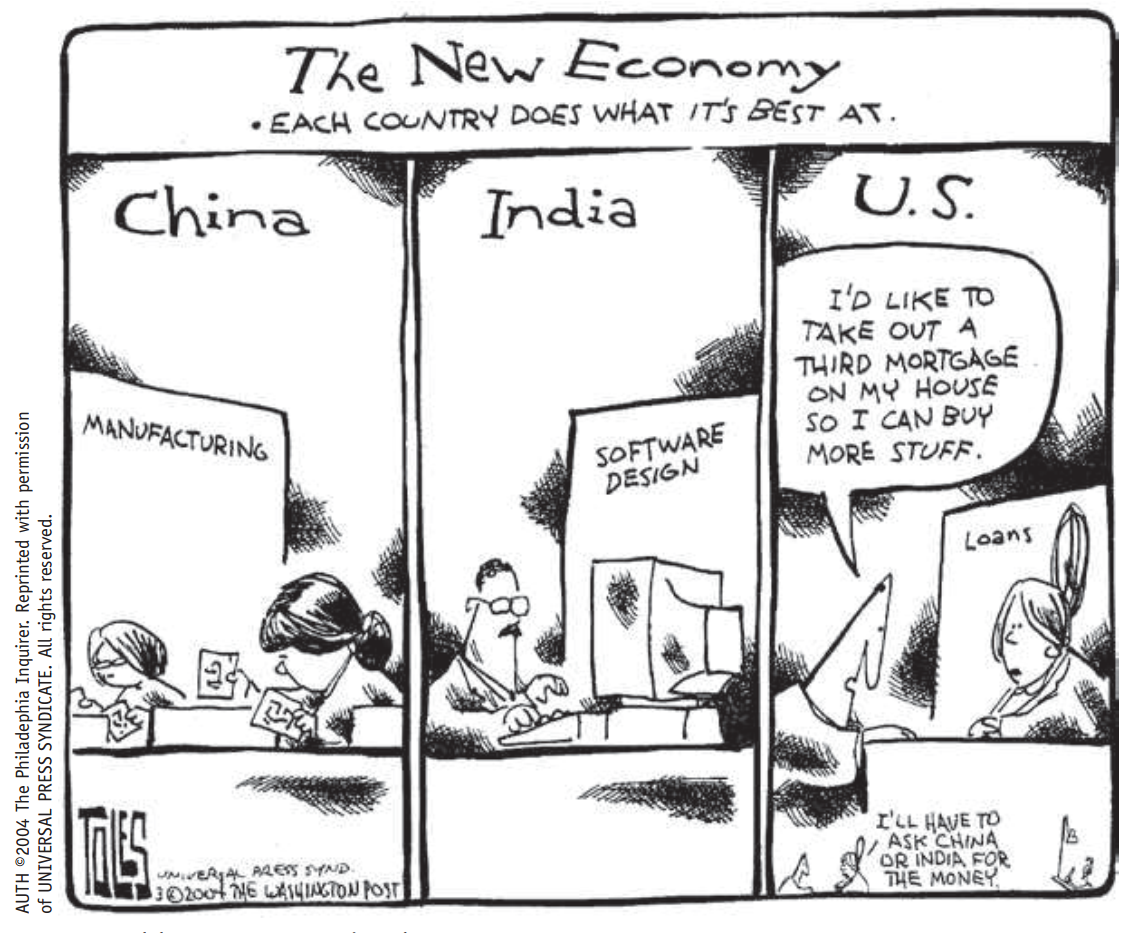
\includegraphics[scale=0.35]{fig/bop/beyondbarter.png}
\end{frame}

\begin{frame}{货币}
\begin{columns}
	\begin{column}{0.7\textwidth}
		\begin{block}{约翰$\bullet$斯图亚特$\bullet$穆勒}
			但是,在多数文明国家的交易中,还保留着如此多的原始风尚,以致几乎所有独立的国家都选择一种他们自己特有的\structure{货币}来昭示他们的民族性,就给他们自己和他们的邻国都带来了不便.
		\end{block}
	\begin{itemize}
		\item 为什么会有货币这种事物的存在,它是谁的杰作?
		\item 在全球化的今天,为什么各个国家不统一货币?
		\item 货币与货币之间币值变化的原因和结果是什么?
		\item 除了民族自豪感之外,一国是从拥有自己的货币中获利呢,还是受损?
	\end{itemize}
	\end{column}
		\begin{column}{0.3\textwidth}
		\centering
		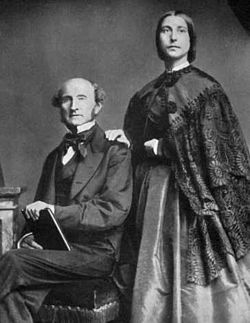
\includegraphics[scale=2]{fig/bop/mill}
	\end{column}
\end{columns}
	
\end{frame}

\begin{frame}{金融}
\begin{columns}
	\begin{column}{0.6\textwidth}
		\begin{block}{波洛尼厄斯(莎士比亚悲剧《哈姆雷特》中的人物}
			不要借钱给别人,也不要向别人借钱;借钱给别人会让你人财两次,向别人借钱会让你挥霍无度,
		\end{block}
	\end{column}
	\begin{column}{0.4\textwidth}
		\centering
		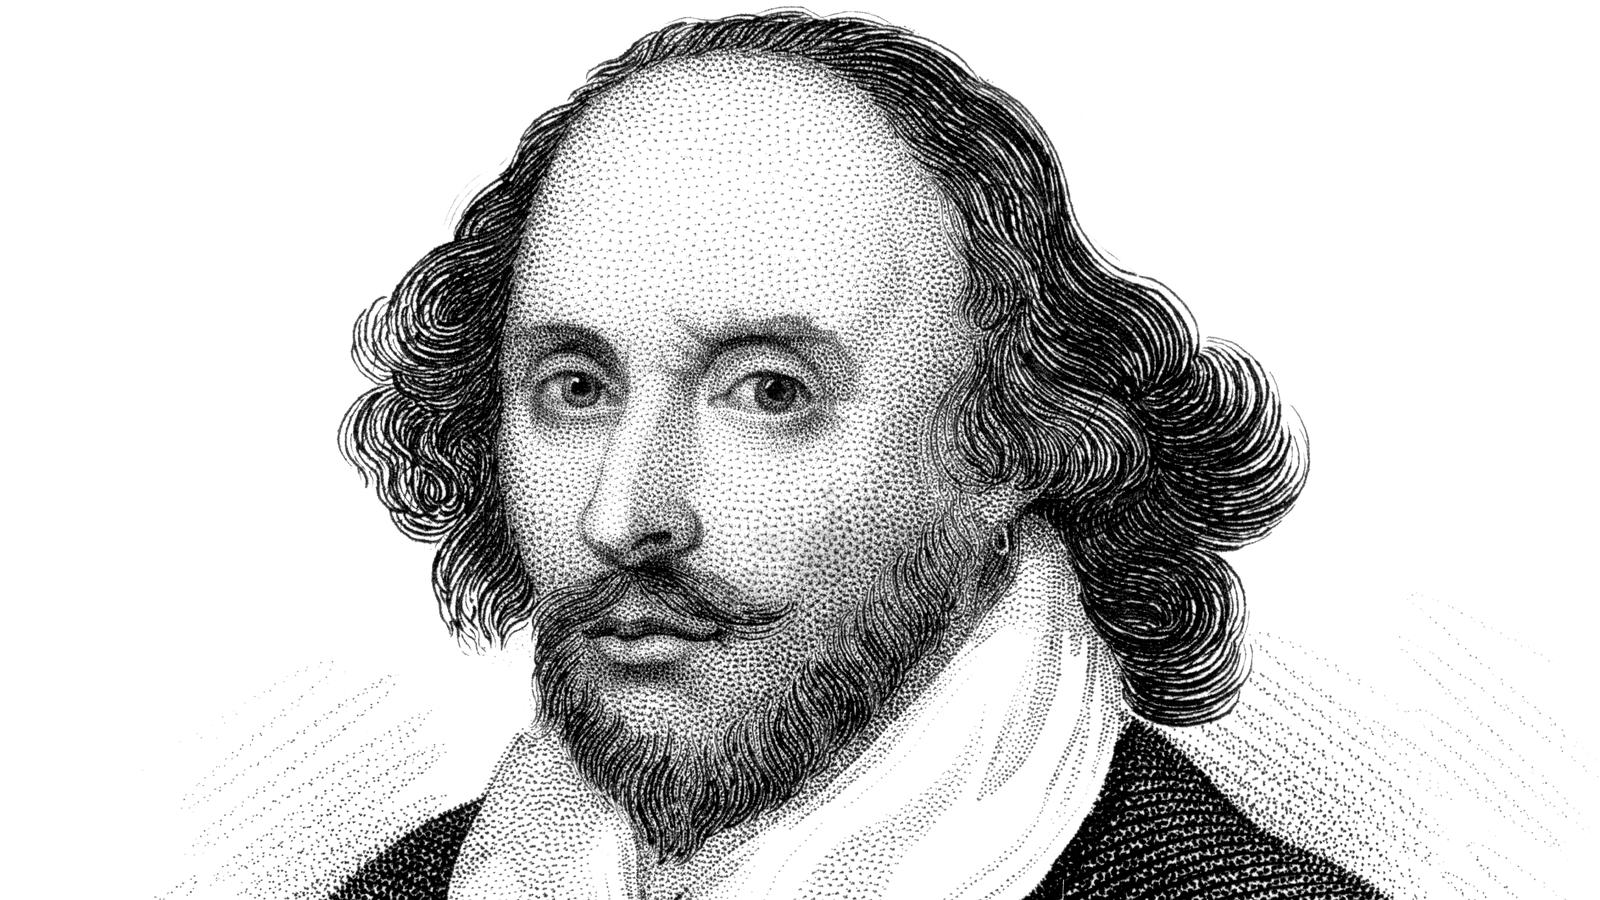
\includegraphics[scale=0.5]{fig/bop/shake}
	\end{column}
\end{columns}
\begin{itemize}
	\item 如果莎士比亚笔下的波洛尼厄斯,能够见识到当今中国和美国不断攀升的外债,他一定会感到沮丧
	\item 当今的全球金融经济中,国际金融交易规模已经达到了前所未有的水平
	\item 为什么会产生这些交易?它们起到了什么作用?是谁向谁放贷?为什么要放贷?
	\item 为什么有些债务偿还了而有些却没有,
	\item 金融的自由流动是经济利益的源泉吗?那么又有什么潜在的经济代价?

\end{itemize}	
\end{frame}

\begin{frame}{政策}
\begin{columns}
	\begin{column}{0.3\textwidth}
		\begin{block}{托马斯$\bullet$杰斐逊}
			总之,历史就只告诉我们一件事:政府有多坏
		\end{block}
	\end{column}
	\begin{column}{0.7\textwidth}
		\centering
		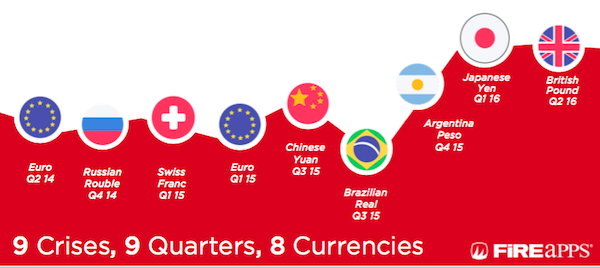
\includegraphics[scale=0.5]{fig/bop/currency}
	\end{column}
\end{columns}
\begin{itemize}
	\item 一个热衷借债的政府一定是坏政府吗?
	\item 为什么人民币走在了国际化的道路上,而有些国家的货币却走在通往地狱的道路上?
	\item 在政府治理的最差的国家里,贫困,投资不足,恶性通货膨胀,经济危机以及债务问题屡屡发生,如何理解这些严重的经济失灵?
	\item 如何评价政府在货币和财政政策?或是在汇率和资本流动性方面作出比较单调的选择呢?有唯一正确的答案吗?
	
\end{itemize}	
\end{frame}

\begin{frame}{Goodbye micro foundations}

\begin{itemize}
	\item Our first trade models
	\begin{itemize}
		\item Stark and simple
		\item General equilibrium
		\item A real economy -- no money!
	\end{itemize}
	\item Models in the remainder of course
	\begin{itemize}
		\item Partial equilibrium
		\item Equilibrium conditions:
		\begin{enumerate}
			\item Interest rate parity
			\item Law of one price
		\end{enumerate}
	\end{itemize}
	\item Text: Micro vs Macro
	\begin{itemize}
		\item A little more complicated than that\dots
	\end{itemize}
\end{itemize}

\end{frame}

\begin{frame}{Why partial equilibrium?}

\begin{itemize}
\item Easier to analyze some important topics
\item Our general equilibrium models abstracted from
\begin{enumerate}
	\item Unemployment
	\item Saving
	\item Trade imbalances
	\item Money
\end{enumerate}

\end{itemize}

\end{frame}

\section{National Income Accounting}

\frame{% how to print
	\frametitle{}
	\begin{center}
		\textcolor{blue}{Chapter 13: National Income Accounting and the Balance of Payments }
	\end{center}
}



\frame{
\frametitle{Gross National Product}
\begin{itemize}
\item Definition from textbook: 
\begin{itemize}
\item \textcolor{red}{The value} of all final goods and services produced by the country's factors of production and sold on the market in a given time period
\end{itemize}
\item The value in common terms -- often current national currency

\item amount of expenditure by buyers ($C+I+G+\textcolor{blue}{CA}$)= amount of income for sellers ($F\left(factors\right)$) = value of production ($Y$)
\end{itemize}
}

\frame{
\frametitle{Gross National Product}
\begin{itemize}
\item Definition from textbook: 
\begin{itemize}
\item The value\textcolor{red}{ of all final goods and services} produced by the country's factors of production and sold on the market in a given time period
\end{itemize}
\item Only final goods are counted, not intermediates
\item Count only the sale of the textbook, not the sale of the paper to the bookmaker
\item Final goods can also be "investment" like production machines
%\item amount of expenditure by buyers ($C+I+G+\textcolor{blue}{CA}$)= amount of income for sellers ($F\left(factors\right)$) = value of production ($Y$)
\end{itemize}
}

\frame{
\frametitle{Gross National Product}
\begin{itemize}
\item Definition from textbook: 
\begin{itemize}
\item The value of all final goods and services \textcolor{red}{produced by the country's factors of production} and sold on the market in a given time period
\end{itemize}
\item The final goods must have been produced using factors of production owned by nationals
\begin{enumerate}
\item Land (resources)
\item Labor (human capital)
\item Capital (machines, buildings, etc)
\end{enumerate}
\item Production does not have to take place within the country
%\item amount of expenditure by buyers ($C+I+G+\textcolor{blue}{CA}$)= amount of income for sellers ($F\left(factors\right)$) = value of production ($Y$)
\end{itemize}
}

\frame{
\frametitle{Gross National Product}
\begin{itemize}
\item Definition from textbook: 
\begin{itemize}
\item The value of all final goods and services produced by the country's factors of production \textcolor{red}{and sold on the market in a given time period}
\end{itemize}
\item Only count final goods that are sold in the relevant year 
\item Do not count sale of used textbooks!
\item Sale of previously manufactured stuff is just exchange, not production
\item Caution: Inventories are counted as a firm selling to itself
%\item amount of expenditure by buyers ($C+I+G+\textcolor{blue}{CA}$)= amount of income for sellers ($F\left(factors\right)$) = value of production ($Y$)
\end{itemize}
}

\frame{
\frametitle{Gross National Product}
\begin{itemize}
\item Definition from textbook: 
\begin{itemize}
\item The value of all final goods and services produced by the country's factors of production and sold on the market in a given time period
\end{itemize}
\item Ex: Fish caught in pearl river and sold in a Xueren restaurant
\begin{itemize}
\item Restaurant buys fish from fisherman -- \emph{not} part of GNP
\item Consumer buys restaurant service, incl. fish -- part of GNP
\end{itemize}
\item Ex: SOE company goes public
\begin{itemize}
\item Investors buy stocks from firm -- \emph{not} part of GNP
\item Investors buy stocks from each other -- \emph{not} part of GNP
\item Commission charges collected by investment bank -- part of GNP
\end{itemize}
\item Ex: Chinese company opens factory in America 
\begin{itemize}
\item Sales of factory are part of GNP (less the wages paid to American labor)
\end{itemize}

%\item amount of expenditure by buyers ($C+I+G+\textcolor{blue}{CA}$)= amount of income for sellers ($F\left(factors\right)$) = value of production ($Y$)
\end{itemize}
}

\frame{
\frametitle{Gross National Product (GNP)}
\begin{itemize}
\item Often separate GNP by ultimate use of production
\end{itemize}
\begin{center}
$GNP=C+I+G+CA$
\end{center}
where
\begin{itemize}
\item $C$ is consumption
\item $I$ is investment
\item $G$ is government purchases
\item $CA$ is current account balance (exports minus imports) 
\item \textcolor{red}{What's the difference of GDP?}
\item Let's talk about these categories
\end{itemize}
}

\frame{
\frametitle{Gross National Product, ultimate use categories}
\begin{center}
$GNP=C+I+G+CA$
\end{center}
\begin{itemize}
\item Consumption
\begin{itemize}
\item Portion of production expended in satisfying current wants
\item Examples: Movie tickets, food, dental work, and washing machines
\item Largest share of production, 60-70\% in US. How much in China?
\end{itemize}
\end{itemize}
}

\frame{
\frametitle{Gross National Product, ultimate use categories}
\begin{center}
$GNP=C+I+G+CA$
\end{center}
\begin{itemize}
\item Investment
\begin{itemize}
\item Any good or service which is used for future production
\item Examples: Machinery for a factory, the newest word processor
\item \emph{Does not} include household ``investment'', or purchases of bonds or shares
\item If company sells bond and uses cash to buy machinery, it is counted as investment
\item The sale of a bond between two people is just an exchange, not production
\end{itemize}
\end{itemize}
}

\frame{
\frametitle{Gross National Product, ultimate use categories}
\begin{center}
$GNP=C+I+G+CA$
\end{center}
\begin{itemize}
\item Government purchases
\begin{itemize}
\item Any good or service ultimately used by the government
\item Examples: new fighter jet, highway repair, basic research 
\item Some countries (China) divide this into:
\begin{itemize}
	\item Government consumption (ex: military)
	\item Government investment (ex: highway repair)
\end{itemize}
\end{itemize}
\end{itemize}
}

\frame{
\frametitle{Gross National Product, ultimate use categories}
\begin{center}
$GNP=C+I+G+CA$
\end{center}
\begin{itemize}
\item \structure{Current account} balance
\begin{itemize}
\item $CA = EX - IM$
\item $EX =$ goods and services produced by Chinese factors and used abroad
\item $IM =$ goods and services produced by Foreign factors and used in China
\end{itemize}
\end{itemize}
}

\frame{
\frametitle{Gross National Product, ultimate use categories}
\begin{center}
$GNP=C+I+G+CA$
\end{center}
\begin{itemize}
\item Current account balance difference between exports and imports
\item $>0$ is \emph{current account surplus}, $<0$ is \emph{current account deficit}
\item Surplus means a country is lending, deficit means borrowing
\item Current account balance is change in net foreign wealth
\end{itemize}
}

\frame{
\frametitle{Gross National Product, ultimate use categories}
\begin{center}
$GNP=C+I+G+CA$
\end{center}
\begin{itemize}
\item Takeaway
\begin{itemize}
\item GNP is (the value of) stuff produced in a country in a year
\end{itemize}
\end{itemize}
}

\frame{
\frametitle{Gross National Product, three details}
\begin{itemize}
\item Three more details from the textbook 
\begin{enumerate}
\item National product vs national income
\item Capital depreciation and international transfers
\item GNP vs GDP
\end{enumerate}
\end{itemize}
}

\frame{
\frametitle{National Product vs. National Income}
\begin{itemize}
\item The value of production ulimately reaches owners of a factor
\item Thus national income should equal national product
\item Almost\dots
\end{itemize}
}

\frame{
\frametitle{National Product vs. National Income}
\begin{enumerate}
\item Capital depreciation like a reduction in the wealth of owners of capital 
\begin{itemize}
\item Needs to be subtracted from production to get income 
\item GNP net of depreciation is called Net National Product (NNP)
\end{itemize}
\item Unilateral transfers
\begin{itemize}
\item Sometimes a country gives goods or services to another country
\item Needs to be added to production to get national income
\end{itemize}
\end{enumerate}
}

\frame{
\frametitle{Gross Domestic Product}
\begin{itemize}
\item GDP has replaced GNP as the most common headline figure in national accounts 
\item Only one difference
\begin{itemize}
\item GDP is the product of all factors in a country, regardless of the owners 
\item GNP is the product of all factors owned by people from a country, regardless of production location
\end{itemize}
\item Ex: If a British firm owns a factory in China
\begin{itemize}
\item The product is part of China's GDP, but not GNP
\end{itemize}
\end{itemize}
}

\frame{
\frametitle{U.S. GNP by use}

\begin{figure}
\centering
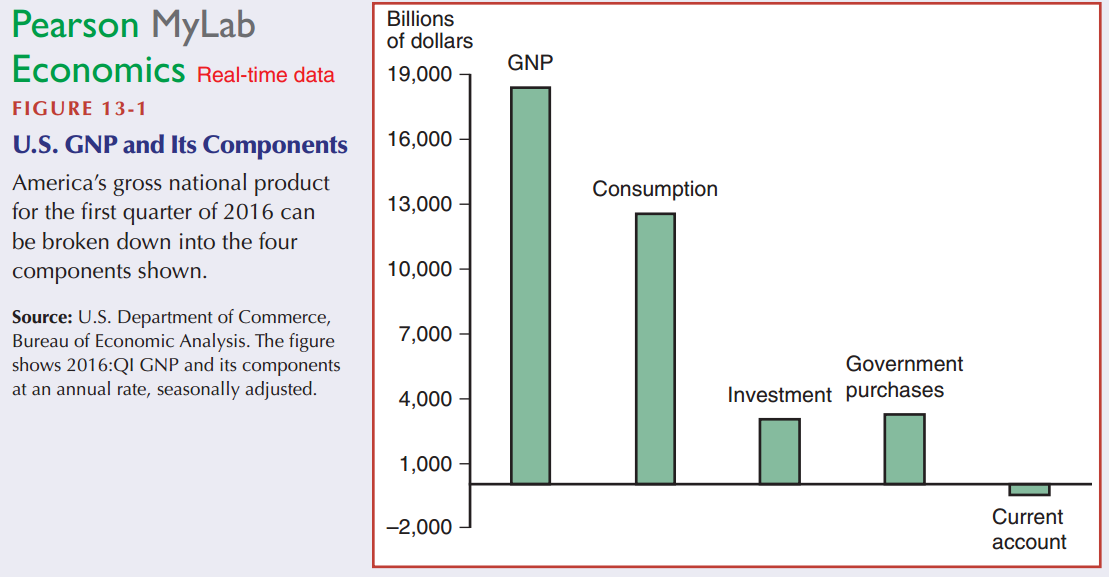
\includegraphics[scale=0.5]{fig/bop/gnp_us.png}
\end{figure}
\begin{itemize}
	\item How would China be different?
\end{itemize}
}

\frame{
	\frametitle{Composition of China GDP}
	\begin{figure}
		\centering
		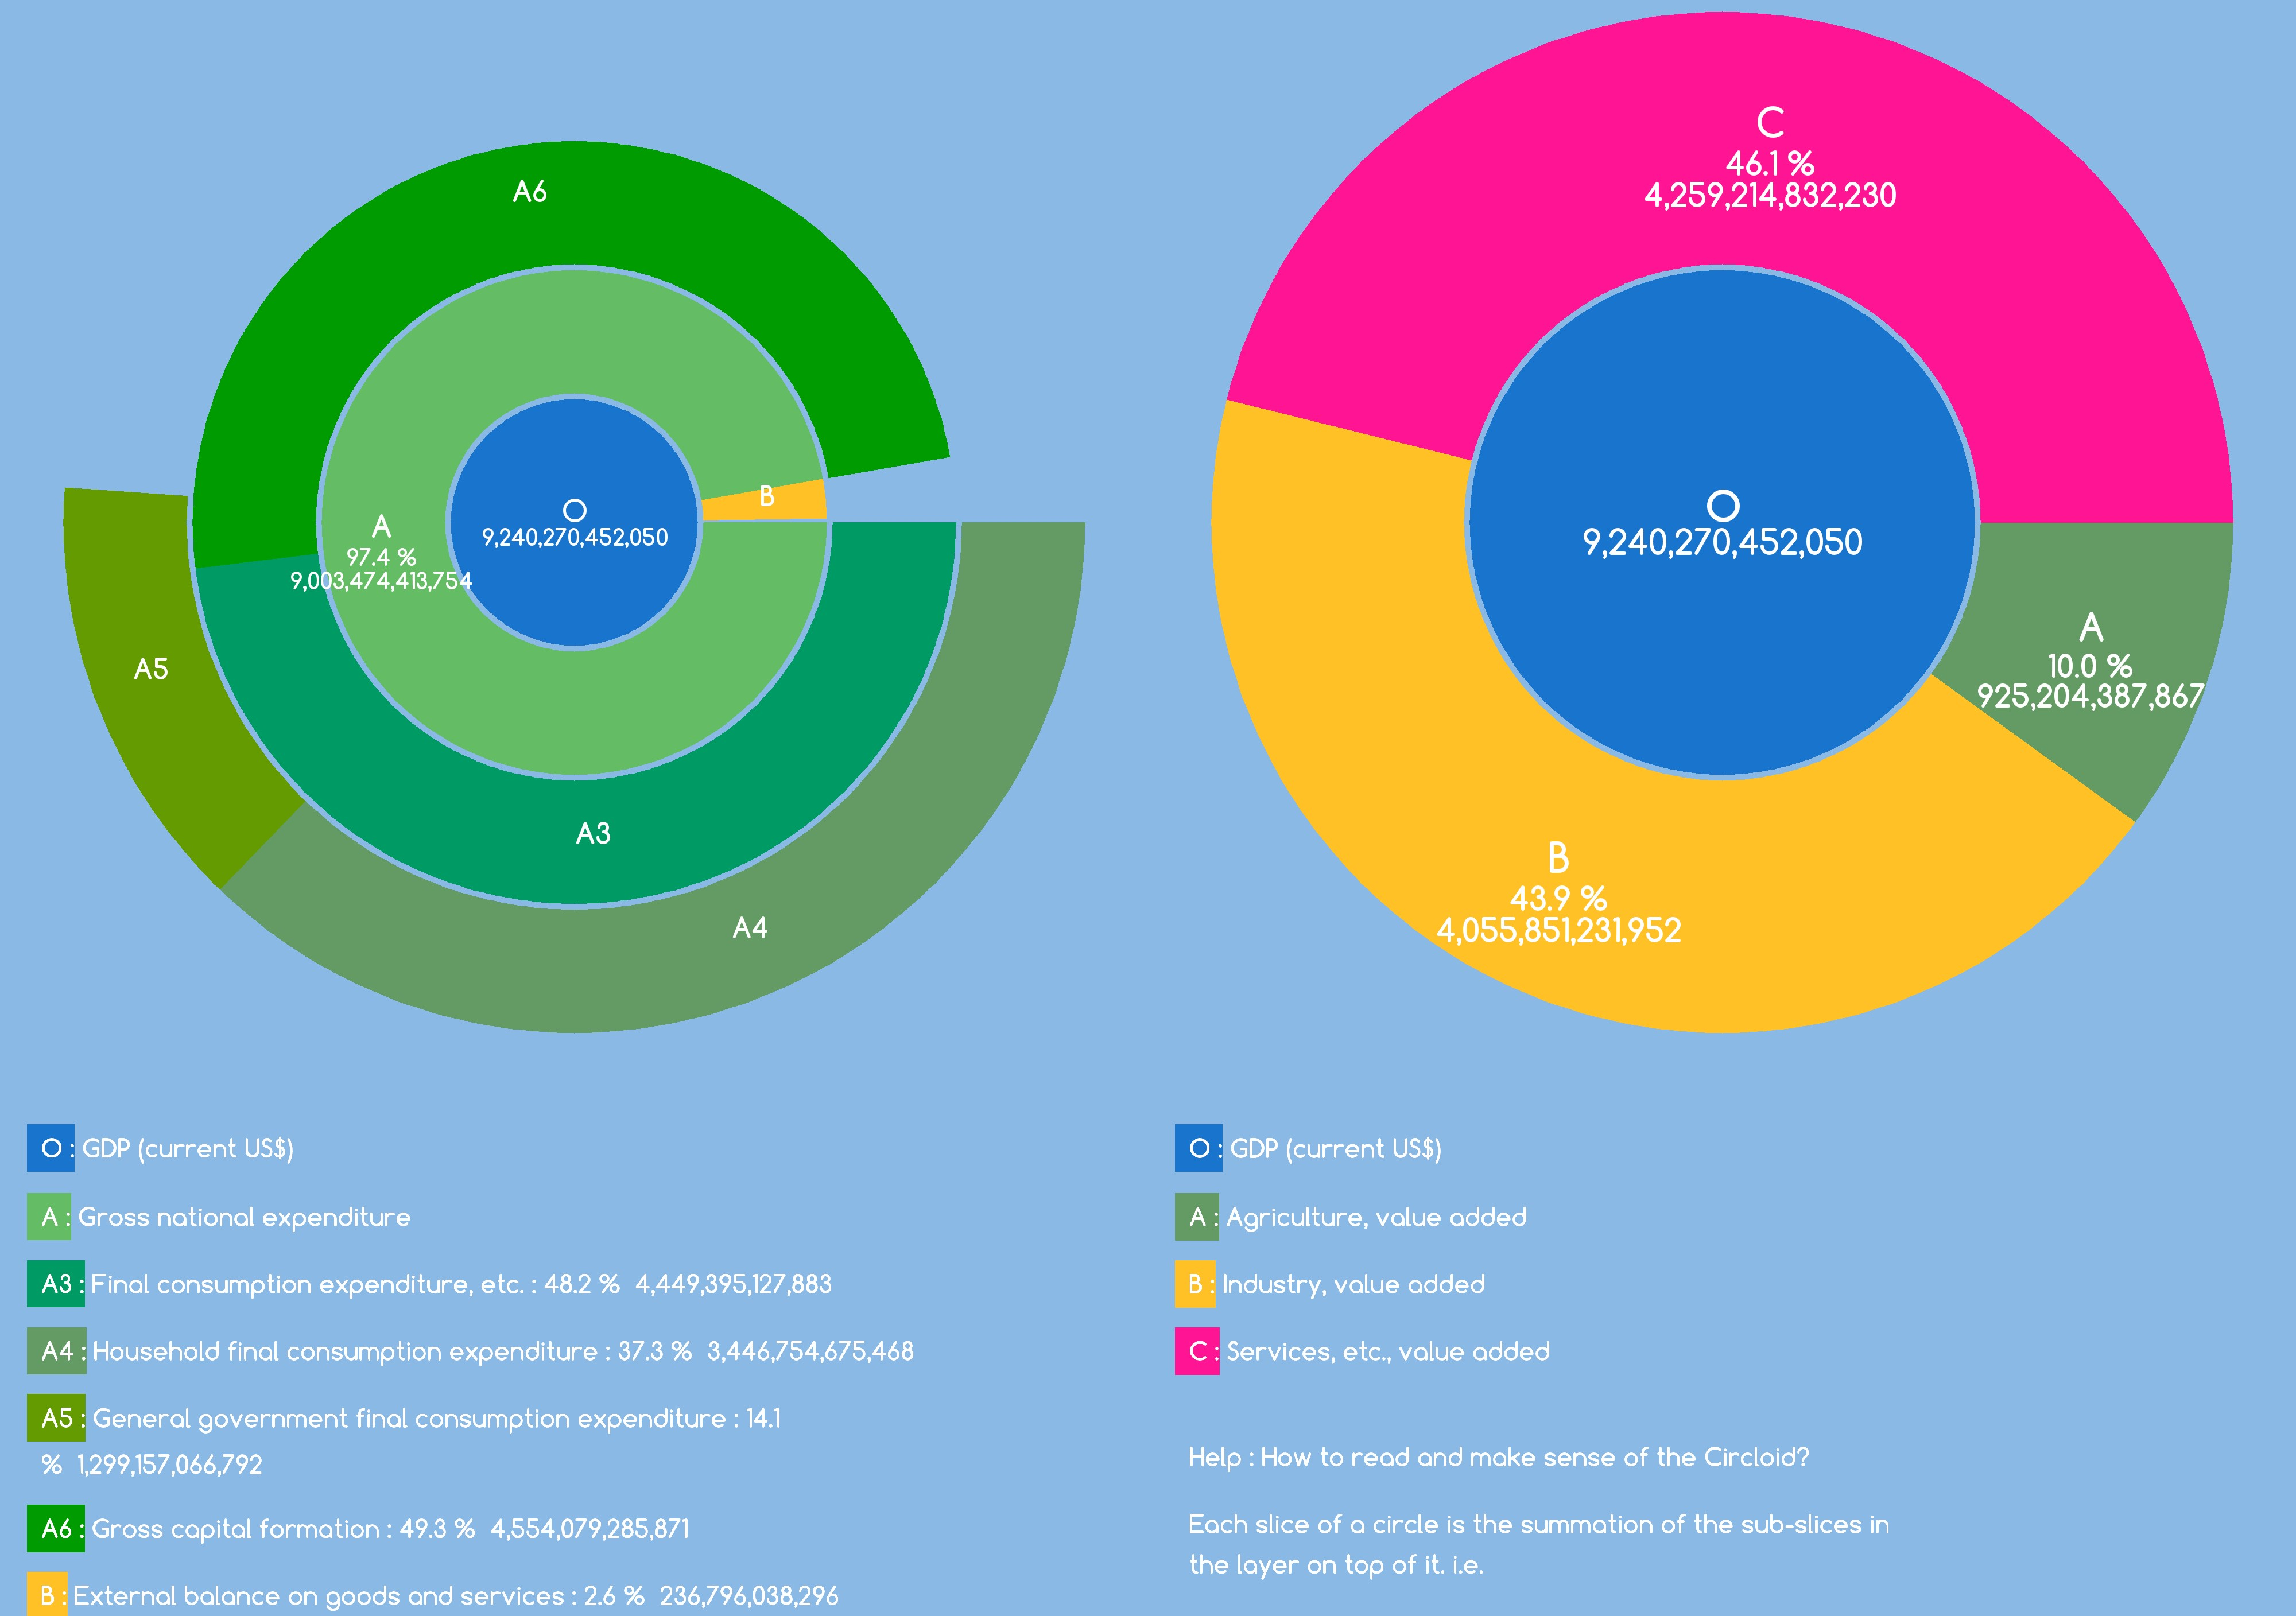
\includegraphics[scale=0.09]{fig/bop/chinagdp.jpg}
	\end{figure}
}

\frame{
\frametitle{More on the Current Account}
\begin{center}
$CA = EX - IM  = Y-  \left(C + I + G \right)$
\end{center}
When production > domestic expenditure, exports > imports: current account > 0 and trade balance > 0
\begin{itemize}
\item if $Y> \left(C + I + G \right) \Rightarrow EX > IM \Rightarrow CA>0$ (surplus)
\item if $Y< \left(C + I + G \right) \Rightarrow EX < IM \Rightarrow CA<0$ (deficit)
\end{itemize}
World production must equal world consumption, investment, and government purchases
\begin{itemize}
\item Globally, deficits and surpluses must balance
\item Some countries often borrowers, others often lenders: \textbf{global imbalances}
\end{itemize}}

\frame{
\frametitle{International Investment Position}
\begin{itemize}
\item The stock of net foreign wealth
\end{itemize}
\centering
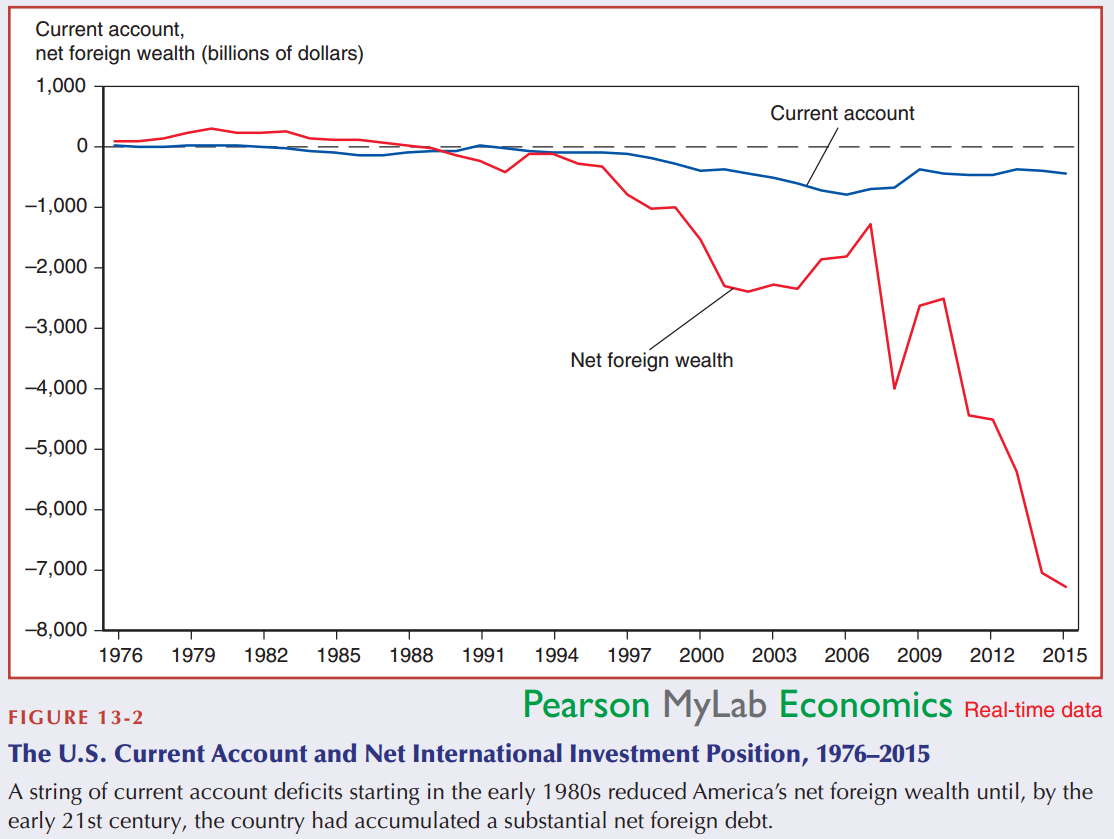
\includegraphics[scale=0.3]{fig/bop/iip_us.png}
\begin{itemize}
\item Why is net foreign wealth so volatile?
\item U.S. Debt Visualized: How It Literally Stacks Up
\url{https://www.zerohedge.com/news/2017-03-05/visualizing-us-debt-ceiling-100-bills}
\end{itemize}
}

\frame[plain]{
\frametitle{Deficits and Surpluses: The Balance of Payments (Source: IMF, International Financial Statistics)}
\begin{columns}
	\begin{column}{0.6\textwidth}
		\begin{figure}
			\centering
			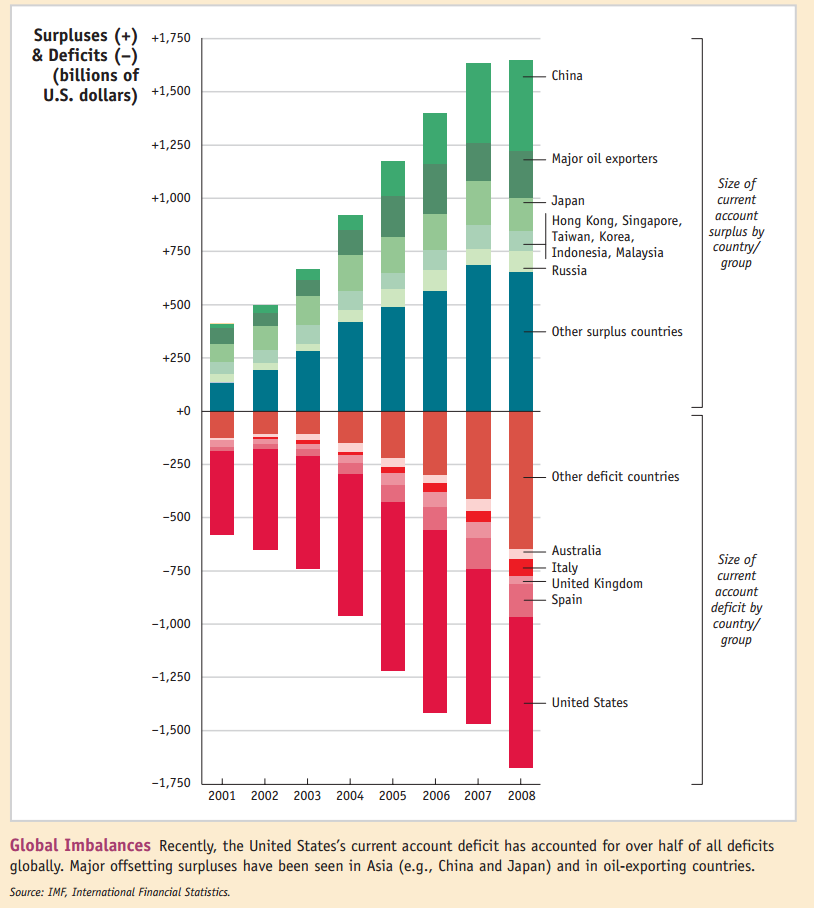
\includegraphics[scale=0.4]{fig/bop/imbalance_imf.png}
		\end{figure}
	\end{column}
	\begin{column}{0.4\textwidth}
	\begin{itemize}
		\item 各种不同国际经济交易是如何造成经常账户不平衡的?
		\item 这些不平衡如何通过金融手段得以解决?
		\item 造成这些不平衡的原因是什么?为什么有些国家会盈余,有些国家会赤字?
		\item 从长远来看,一个经济运行运行良好的国家,他的经常账户不平衡会起到什么作用?
		\item 为什么这些不平衡会是许多政策争论的焦点?
	\end{itemize}
\end{column}
\end{columns}

}

\frame{
\frametitle{National Saving}
\begin{itemize}
\item Define national savings as:
\begin{equation*}
S=Y - C - G
\end{equation*}
\item GNP identity:
\begin{equation*}
Y =  C + I + G + CA
\end{equation*} 
\item Combine the two:
\begin{equation*}
\implies       S - CA =  I
\end{equation*}
\item Investment can be financed by:
\begin{enumerate}
\item Putting off consumption (pay today)
\item Borrowing from abroad (pay tomorrow)
\item Current account sometimes called \emph{net foreign investment}
\end{enumerate}
\end{itemize}
}

\frame{
\frametitle{National Saving: Private vs government}
\begin{center}
$S=Y -C -G $
\end{center}
\begin{center}
$S=\left(Y -C - T\right) + \left(T - G\right)$
\end{center}
\begin{center}
$S=S^{p} + S^{g}$
\end{center}
}

\frame{
\frametitle{National Saving: Private vs government}
\begin{itemize}
\item Combining our two definitions of saving:
\begin{equation*}
S = I + CA = S^{p} + S^{g}
\end{equation*}
\begin{equation*}
S^{p} = I + CA - S^g 
\end{equation*}
\begin{equation*}
S^{p} = I + CA + \left(G - T\right)
\end{equation*}
\item Private saving is used for: 
\begin{enumerate}
\item Investment at home
\item Investment abroad
\item Purchasing government debt(政府预算赤字)
\end{enumerate}
\end{itemize}
}

\begin{frame}{小结}
\begin{itemize}
\item National Income Accounts
\begin{itemize}
\item $GNP: Y = C + I + G + CA$
\item Only count stuff produced by factors owned by nationals
\item Investment can be funded by foreign borrowing
\end{itemize}
\item Next: Balance of Payment Account
\begin{itemize}
\item Tracks credits and liabilities between countries 
\item Similar to a balance sheet from accounting
\end{itemize}
\end{itemize}
\end{frame}

\section{Balance of Pyaments Accounting}

\begin{frame}{The Flow of Payments in a Closed Economy}
	\centering
	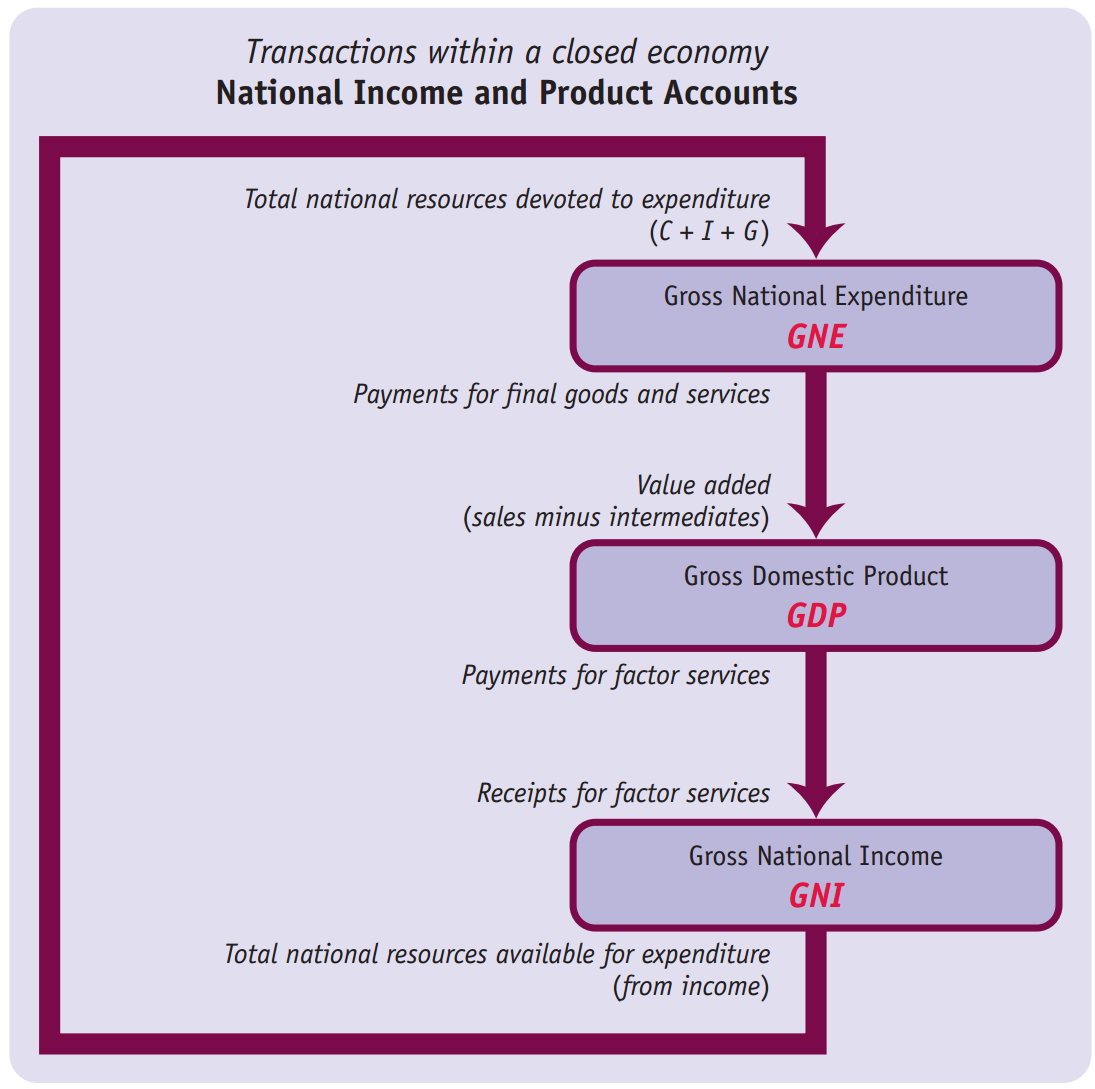
\includegraphics[width=0.45\textwidth]{fig/bop/closegdp.png}
\end{frame}

\begin{frame}{The Flow of Payments in a Open Economy}
\centering
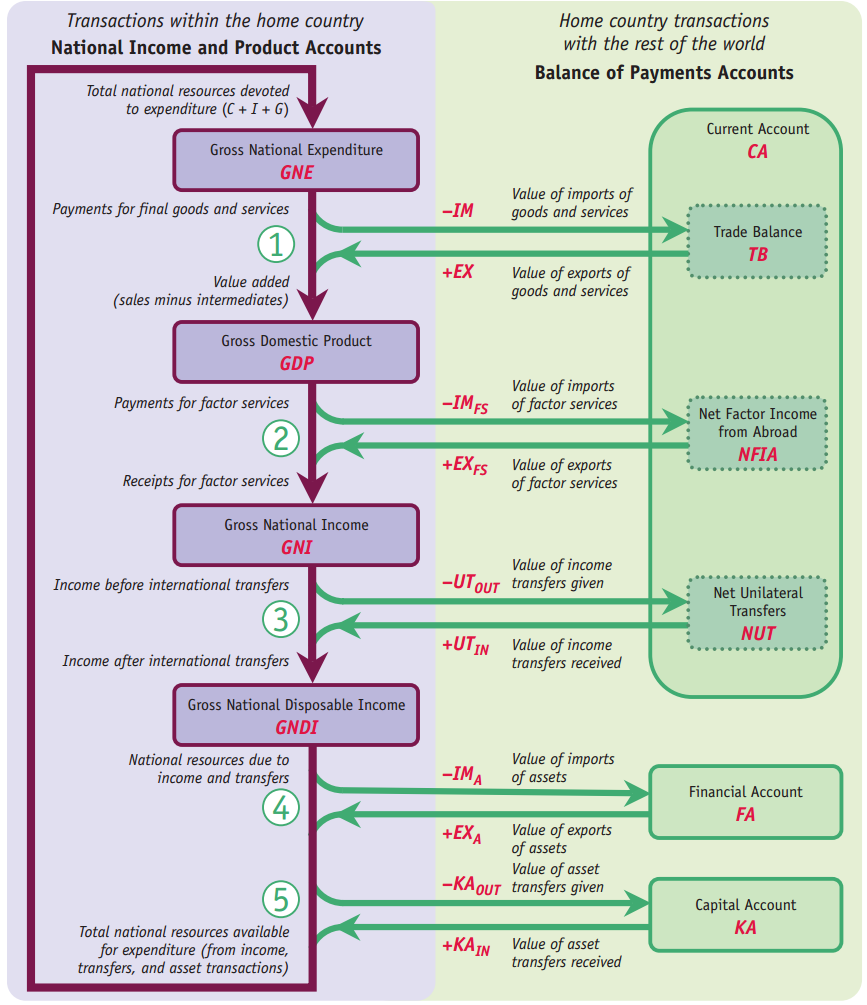
\includegraphics[width=0.4\textwidth]{fig/bop/opengdp.png}
\end{frame}

\frame{
	\frametitle{Balance of Payments Accounts }
	\begin{itemize}
		\item Two types of transactions:
		\begin{enumerate}
			\item Credit if a foreigner pays a native
			\item Debit if a native pays a foreigner
		\end{enumerate}
		\item A \emph{Financial Asset} holds wealth: stocks, bonds, debt, etc
		\item current account + financial account + capital account = 0
		\begin{enumerate}
			\item \textbf{current account}:  tracks flows of goods and services (imports and exports)
			\item \textbf{financial account}:  tracks flows of financial assets (financial capital)
			\item \textbf{capital account}:  flows of special categories of assets:  typically intangible assets like debt forgiveness, copyrights and trademarks.
		\end{enumerate}
	\end{itemize}
}

\begin{frame}{国际收支平衡表}
	\begin{itemize}
		\item 按照一定的编制原则和格式,排列组合特定时期内一国经济主体与他国经济主体之间的各项经济交易
		\item 是全面系统地记录和总结一国国际收支状况的统计报表
		\item 是反映一国对外经济发展、偿债能力等的重要文件,也是各国制定开放经济宏观经济政策的重要依据
		\item 各国编制BOP需要遵照IMF制定的规则——BPM,latest edition(BPM6) was issued in 2010
		
	\end{itemize}
\end{frame}

\begin{frame}{国际收支平衡表编制原则}
\begin{enumerate}
	\item 复式记账原则
	\begin{itemize}
		\item 任意国际经济交易都应在借贷双方同时反映
	\end{itemize}
	\item 权责发生制原则
	\begin{itemize}
		\item 交易的记录时间以所有权转移为标准
	\end{itemize}
	\item 市场价格原则
	\begin{itemize}
		\item 单一记账货币原则
	\end{itemize}
	\item 单一货币记账原则
	\begin{itemize}
		\item 可以是外币,也可以是本币
		\item 中国一般提供美元、SDR和人民币的多种版本
	\end{itemize}
\end{enumerate}
\end{frame}

\begin{frame}{复式记账原则}
\begin{enumerate}
	\item 会计科目划分为借方和贷方
		\begin{itemize}
		\item 借方科目为资金占用类科目,反映对外支付
		\item 贷方科目为资金来源类科目,反映接受付款
		\item 借方科目增加记“-”,贷方科目增加记“+”
		\end{itemize}
	\item 每一笔对外交易需要同时留下两个记录,金额相同,方向相反
		\begin{itemize}
		\item 借方记录国内居民对国外支付的交易
		\item 贷方记录国内居民接受国外支付的交易
		\end{itemize}	
\end{enumerate}
\end{frame}

\begin{frame}{复式记账实例}
\begin{enumerate}
	\item 某企业向美国出口价值200万美元的服装,进口商将款项汇入指定银行账户	
	\begin{itemize}
		\item 出口创汇,属贷方科目,记“+\$200万”
		\item 持有外国资产,属借方科目,记“-\$200万”

	\end{itemize}
	\item 张三向国外大学汇出100美元留学申请费	
	\begin{itemize}
		\item 为进口服务付汇,属借方科目,记“-\$100”		
		\item 持有外国资产减少,记“+\$100”		
	\end{itemize}	
\end{enumerate}
\end{frame}

\begin{frame}{复式记账实例}
\begin{enumerate}
	\item 强调居民与非居民的交易而不是资金收付	
	\begin{itemize}
		\item 国际收支$\neq$外汇收支
	\end{itemize}
	\item 考察流量而不是存量,记录发生额而不是持有额
		\begin{itemize}
		\item 国际收支平衡表支$\neq$国家资产负债表				
	\end{itemize}
	\item 理论上全球国际收支差额可以彼此抵消,但各个国家的表现并不如此
\begin{itemize}
	\item 某些国家存在巨大的收支失衡		
\end{itemize}
	\item 国际收支经常不平衡,但国际收支平衡表永远账面平衡
\begin{itemize}
	\item 设置“储备资产变动”和“错误与遗漏”项目				
\end{itemize}
\item 	国际收支是个事后的概念
\end{enumerate}
\end{frame}

\begin{frame}{Global Imbalances}
\centering
\includegraphics[width=0.65\textwidth]{fig/bop/globalimbalances.png}
\end{frame}

\frame{
	\frametitle{Example 1: US imports fax machine}
	\begin{itemize}
		\item US imports fax machine from Italy
		\item Italian firm deposits USD in US bank
	\end{itemize}
	\begin{figure}
		\centering
		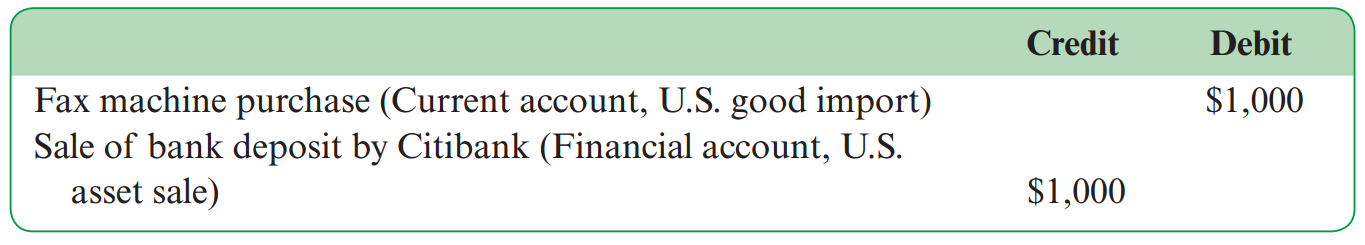
\includegraphics[width=0.85\textwidth]{fig/bop/num1.png}
	\end{figure}
}

\frame{
	\frametitle{Example 2: US tourist buys French lunch}
	\begin{itemize}
		\item US tourist buys lunch in Paris
		\item Pays with US credit card
	\end{itemize}
	\begin{figure}
		\centering
		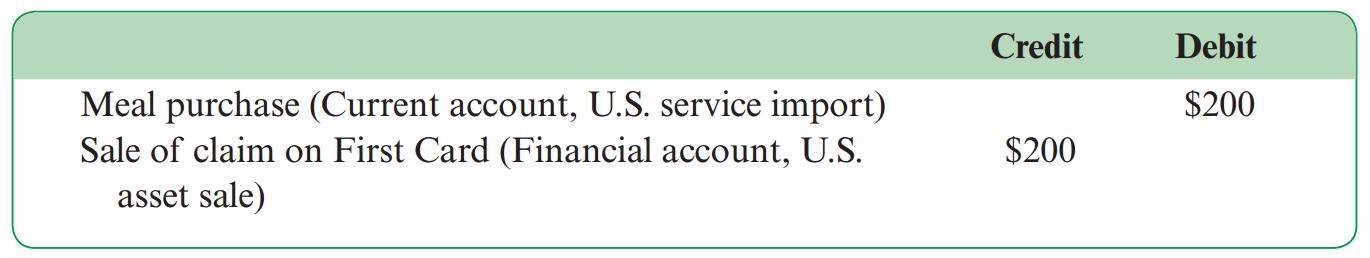
\includegraphics[width=0.85\textwidth]{fig/bop/num2.png}
	\end{figure}
}

\frame{
	\frametitle{Example 3: American buys share of British Petroleum}
	\begin{itemize}
		\item American buys a share of BP
		\item BP deposits money in American bank
	\end{itemize}
	\begin{figure}
		\centering
		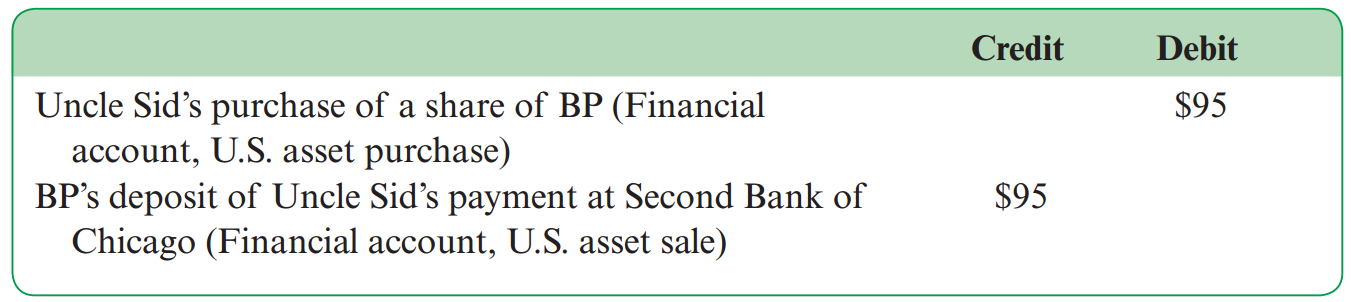
\includegraphics[width=0.85\textwidth]{fig/bop/num3.png}
	\end{figure}
}

\frame{
	\frametitle{U.S. Balance of Payments Accounts for 2015 (billions of dollars)}
	\begin{figure}
		\centering
		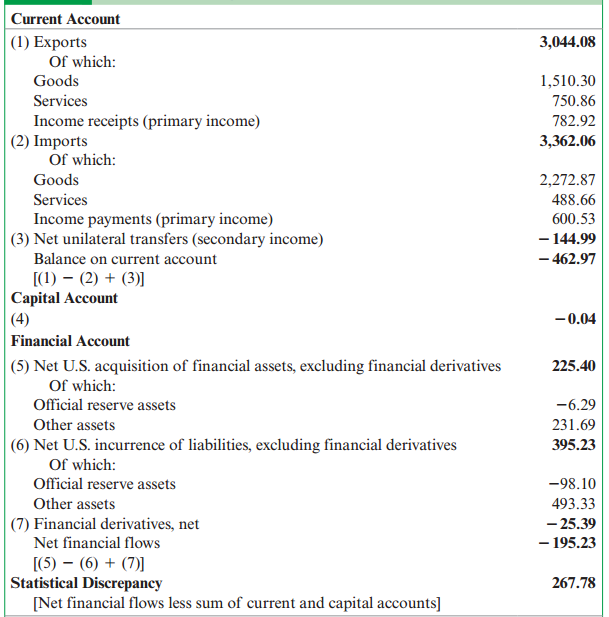
\includegraphics[scale=0.5]{fig/bop/bop_2015.png}
	\end{figure}
}

\frame{
	\frametitle{China Balance of Payments Accounts for 2015 (billions of dollars)}
	\begin{figure}
		\centering
		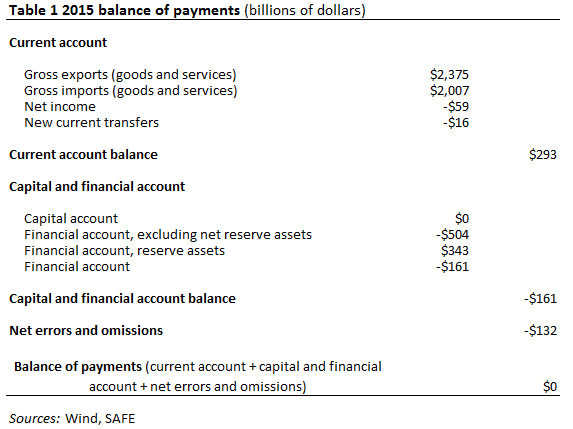
\includegraphics[scale=0.5]{fig/bop/chinabop.png}
	\end{figure}
}

\frame{
	\frametitle{Official reserve assets}
	\begin{itemize}
		\item Central banks hold foreign currency reserves
		\begin{itemize}
			\item Purpose: Insure against macroeconomic fluctuations
		\end{itemize}
		\item These are often American Treasury bills (promises that the American government will pay a dollar tomorrow)
		\item Buying and selling these bills locally allows central banks to affect money supply
	\end{itemize}
}

\frame{
	\frametitle{Expansion of credit end of 20th century}
	\begin{figure}
		\centering
		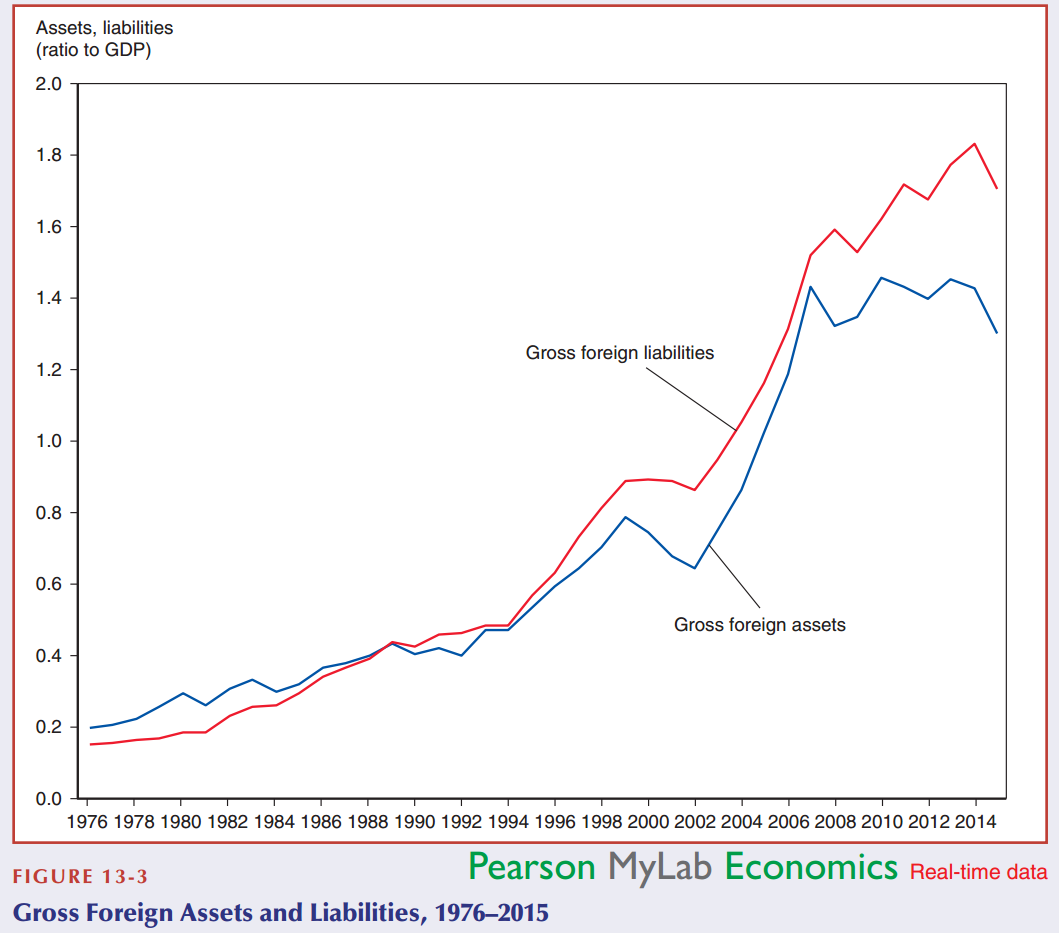
\includegraphics[scale=0.4]{fig/bop/credit_expansion.png}
	\end{figure}
}

\begin{frame}{Takeaways}
\begin{itemize}
	\item National Income Accounts
	\begin{itemize}
		\item $GNP: Y = C + I + G + CA$
		\item Only count stuff produced by factors owned by nationals
		\item Investment can be funded by foreign borrowing
	\end{itemize}
	\item Balance of Payment Account
	\begin{itemize}
		\item Tracks credits and liabilities between countries 
		\item That is, who consumes now and who in the future 
	\end{itemize}
\end{itemize}
\end{frame}


\end{document}